\apendice{Procesado automático de la imagen}

\section{Por procesado de imagen}
Todas las imágenes van hacer un proceso de convolución, con el Kernel especifico en cada caso.

Una convolución es una operación matemática, que no es la multiplicación de matrices tradicional, es el proceso de agregar cada porción de la imagen a sus vecinos locales ponderado por el Kernel. 

Este proceso no solo vale para detectar bordes, tiene estas otras aplicaciones.
\begin{itemize}
\item Detección de bordes.
\item Normalización.
\item Desenfoques y difuminado.
\item Eliminar ruido. 
\end{itemize}

\subsection{Laplace:}
Esta función busca bordes usando el operador de Laplace. En nuestro caso de tamaño 3 ya que se puede especificar el tamaño.

Kernel Laplace \ref{F_k1}.
\begin{table}[]
	\centering
	\caption{Kernel Laplace}
	\label{F_k1}
	\begin{tabular}{|l|l|l|}
		\hline
		0 & 1  & 0 \\ \hline
		1 & -4 & 1 \\ \hline
		0 & 1  & 0 \\ \hline
	\end{tabular}
\end{table}

from skimage.filters import laplace,prewitt\\
bord=laplace(img,ksize=3)

Observaciones:
Como podemos observar no es un método factible para nuestro propósito por lo que no vamos a continuar usándolo.

\subsection{Prewitt:}

Encuentra los bordes usando la transformada de Prewitt.

Kernel Prewitt \ref{F_k2}.
\begin{table}[]
	\centering
	\caption{Kernel Prewitt}
	\label{F_k2}
	\begin{tabular}{|l|l|l|}
		\hline
		1  & 1   & 1 \\ \hline
		0  & 0   & 0 \\ \hline
		-1 & -1  & -1 \\ \hline
	\end{tabular}
\end{table}



Observaciones:
Como podemos ver las grietas en la imagen las detecta bien pero las estrías de dieta son siluetas muy tenues y contiene mucho ruido.


\subsection{Scharr:}
Con este método encontramos los bordes usando la transformada de Scharr.

Kernel HScharr \ref{F_k3}.
\begin{table}[]
	\centering
	\caption{Kernel HScharr}
	\label{F_k3}
	\begin{tabular}{|l|l|l|}
		\hline
		3  & 10  & 3 \\ \hline
		0  & 0   & 0 \\ \hline
		-3 & -10 & -3 \\ \hline
	\end{tabular}
\end{table}
todo ello partido de 16 y para las verticales es la matriz transpuesta. 




Observaciones:
Como podemos ver en la imagen las estrías de dieta son muy tenues pero ligeramente mejores que en la anterior tampoco demasiado pero ligeramente, el método es algo más rápido también pero no obtenemos algo tangible.




\subsection{Sobel:}
Este método busca bordes usando la transformada de Sobel.


Kernel HSobel \ref{F_k4}.
\begin{table}[]
	\centering
	\caption{Kernel HSobel}
	\label{F_k4}
	\begin{tabular}{|l|l|l|}
		\hline
		1  & 2  & 1 \\ \hline
		0  & 0  & 0 \\ \hline
		-1 & -2 & -1 \\ \hline
	\end{tabular}
\end{table}
Todo ello partido de 4 y para las verticales es la matriz transpuesta. 




Observaciones: 
Con este método tal y como podemos observar en la imagen crea más ruido que los anteriores pero también podemos observar la silueta de las estrías de dieta.


\subsection{Roberts:}

Esta función encuentra los bordes usando la operación cruzada de Robert

Kernel Roberts \ref{F_k5}.
\begin{table}[]
	\centering
	\caption{Kernel Roberts}
	\label{F_k5}
	\begin{tabular}{|l|l|}
		\hline
		0  & 1 \\ \hline
		-1 & 0 \\ \hline
	\end{tabular}
\end{table}




Observaciones:
Este método produce mucho ruido y las estrías son líneas demasiado tenues.

\subsection{Kirsch:}
Esta función encuentra los bordes usando el kernel de Kirsch.
para cada dirección.
No estaba implementado en Skimage por lo que he implementado el método.

Kernel g1 \ref{F_k6_1}.
\begin{table}[]
	\centering
	\caption{Kernel g1}
	\label{F_k6_1}
	\begin{tabular}{|l|l|l|}
		\hline
		5  & 5  & 5  \\ \hline
		-3 & 0  & -3 \\ \hline
		-3 & -3 & -3 \\ \hline
	\end{tabular}
\end{table}

Kernel g2 \ref{F_k6_2}.
\begin{table}[]
	\centering
	\caption{Kernel g2}
	\label{F_k6_2}
	\begin{tabular}{|l|l|l|}
		\hline
		5  & 5  & -3  \\ \hline
		5 & 0  & -3 \\ \hline
		-3 & -3 & -3 \\ \hline
	\end{tabular}
\end{table}


Kernel g3 \ref{F_k6_3}.

\begin{table}[]
	\centering
	\caption{Kernel g3}
	\label{F_k6_3}
	\begin{tabular}{|l|l|l|}
		\hline
		5  & -3 & -3  \\ \hline
		5 & 0  & -3 \\ \hline
		5 & -3 & -3 \\ \hline
	\end{tabular}
\end{table}

kernel g4 \ref{F_k6_4}.

\begin{table}[]
	\centering
	\caption{Kernel g4}
	\label{F_k6_4}
	\begin{tabular}{|l|l|l|}
		\hline
		-3  & -3 & -3  \\ \hline
		5 & 0  & -3 \\ \hline
		5 & 5 & -3 \\ \hline
	\end{tabular}
\end{table}
Observaciones:
Este método produce mucho ruido y las estrías son líneas demasiado tenues.
No obstante de los métodos hasta ahora usados es en el que mas aprecian.

\subsection{Autovectores matriz Hessiana:}
Este método consiste en obtener la matriz hessiana y después sus autovectores de la matriz Hessiana y nos devuelve dos matrices la matriz i1 es la matriz con el autovector más largo y la i2 es la matriz con autovector más corto.





Observaciones: 
Como podemos observar en la imagen en escala de grises del autovector de los valores más largos las siluetas de las estrías de dieta son las que más se remarcan sobre un tenue fondo gris pero pudiendo ser observadas por lo que este podría ser un punto de partida.



\subsection{Canny:}

\subsubsection{Eliminando ruido:}
Primero ,obtener los bordes, llamar a una función que elimina el ruido y después al detector de bordes canny, para obtener los bordes.
Los parámetros del canny en como sigma un valor intermedio de 1.4 junto con un umbral bajo, muy bajo, y un umbral alto, también bajo.
Obtenemos una imagen resaltando algunos bordes pero no todo los que queremos ya que no están demasiado marcados.




Observaciones:
Desde esta imagen con bastante ruido ya podemos observar que las más marcadas son detectadas pero no se consiguen diferenciar demasiado bien, pero en comparación con los demás métodos tiene de las mejores salidas aun no siendo buena de ir en esta línea tendiéramos que usar esto.

\subsubsection{Modificando parámetros Canny:}

La segunda opción ha sido usar un detector de bordes Canny solamente modificando sus parámetros pero en esta opción los valores de los umbrales deben ir sin normalizar entre 0 y 1 sino entre 0 y 255.


Observaciones:
Esta imagen detecta menos ruido que con la otra tentativa pero sigue siendo deficiente en cuanto a las líneas ya que aparte de detectar pocas detecta las que realmente no son estrías de dieta. Pero de ir en alguna línea seria por este camino.



\subsection{Gabor:}

Es un filtro linear con un kernel gausiano  que es modulado por un onda sinusoidal plana. Principalmente se usa en visión artificial de clasificación y detección de bordes.
Obtenemos un par de imágenes.



Observaciones:
Este método lo eh probado porque en la obtención de las líneas de sangre en los ojos es lo que se usa para ello pero al no ser líneas continuas y no seguir un patrón no he conseguido buenos resultados. En el filtro real no es tan malo pero en el filtro imaginario es ruido puro.
\subsection{Comparativa Filtros}
Comparativa de todos los filtros \ref{fig:1.1} y \ref{fig:1.2}. 

\subsection{Procesado:}
Partiendo del análisis anterior vamos a juntar los mejores resultados y añadir pasos adicionales para obtener la mascara binaria que mas podamos ajustar a nuestras necesidades.


Pasos del algoritmo \ref{fig:2.1} y \ref{fig:2.2}.
\begin{itemize}
	\item Ecualizar la imagen original:
Así conseguimos que sus histograma este mas repartido por toda la gama de grises y no centrado en un pequeño rango.
	\item Autovectores de la Hessiana:
Obtenemos los autovectores de la matriz Hessiana y nos quedamos con los largos, ya que los autovectores pueden ser los cortos o los largos. 
	\item Sustraemos el fondo a la imagen:
Como la imagen no tiene de nuevo demasiada gama cromatica le sustraemos el fundo para asi quedarnos unicamente con las lineas, al tener ruido aparte de lo que queremos, tendremos mucho ruido.
	\item Binarizamos la imagen:
Como la imagen aun habiendo sustraido el fondo no es binaria hay que aplicarle un treshold o umbral para pasar a blanco o negro, es decir, binarizarla.
	\item Eliminamos el ruido:
Este paso anterior, en estas condiciones de trabajo genera mucho ruido, por lo que tendremos que intentar reducirlo y para ello eliminamos los trozos que son pequeños, esto elimina la mayoría de los puntos de ruido.
	\item Erosionar con operador diamante:
Para suavizar la imagen y evitar que queden lineas finas a modo de antenas, erosionamos la imagen con un operador estructurante en forma de diamante, así conseguimos que pase por la mayoría de las figuras.
	\item Esqueletonizar la imagen:
Una vez tengamos la imagen sin tanto ruido, reducimos el grosor de las lineas para que la función de Hough funcione, así nos detecta las lineas que corresponden a esta mascara binaria.
	\item Eliminar mas ruido:
Este paso anterior vuelve a generar ruido porque algunos trozos se dividen en pequeños segmentos y con la segunda reducción de ruido conseguimos hacerlos desaparecer y quedarnos con las lineas grandes.
\end{itemize}



\begin{figure}
	\begin{subfigure}[c]{.5\linewidth}
	\centering\large 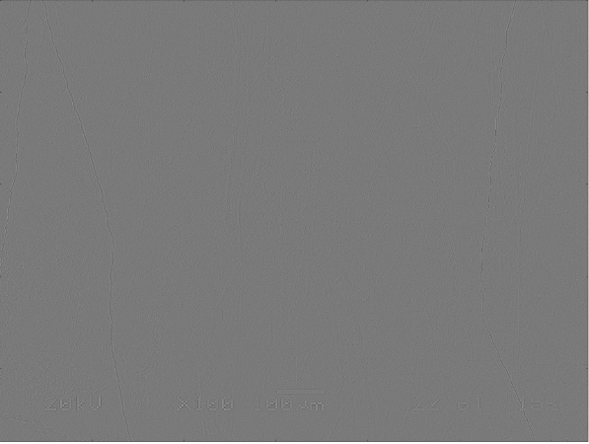
\includegraphics[width=.9\textwidth]{Laplace}
	\caption{Bordes usando Laplace}
	\end{subfigure}%
	\begin{subfigure}[c]{.5\linewidth}
	\centering\large 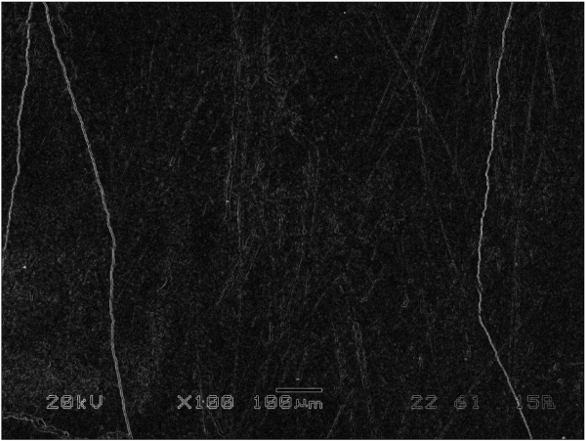
\includegraphics[width=.9\textwidth]{Prewitt}
	\caption{Bordes usando Prewitt}
	\end{subfigure}%

	\begin{subfigure}[c]{.5\linewidth}
	\centering\large 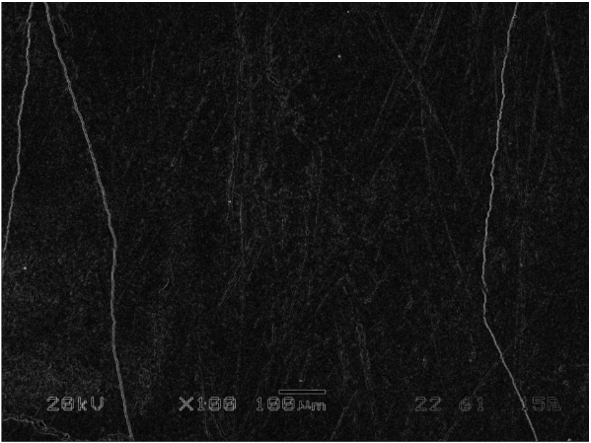
\includegraphics[width=.9\textwidth]{Scharr}
	\caption{Bordes usando Scharr}
	\end{subfigure}%	
	\begin{subfigure}[c]{.5\linewidth}
	\centering\large 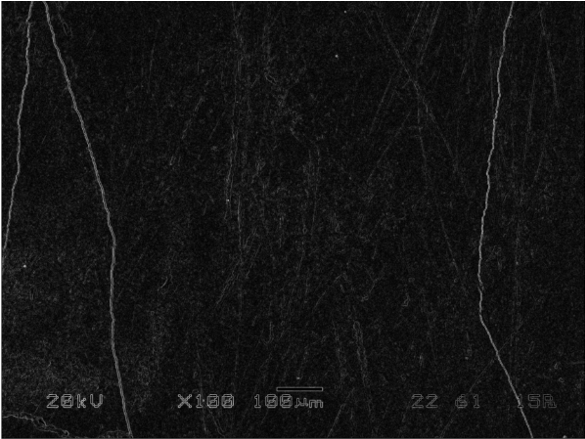
\includegraphics[width=.9\textwidth]{Sobel}
	\caption{Bordes usando Sobel}
	\end{subfigure}%
	
	\begin{subfigure}[c]{.5\linewidth}
	\centering\large 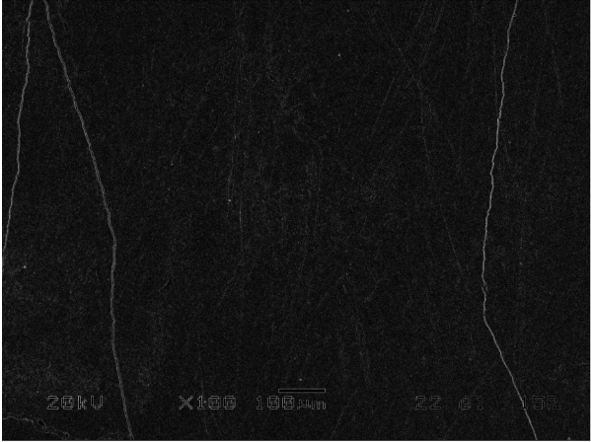
\includegraphics[width=.9\textwidth]{Roberts}
	\caption{Bordes usando Roberts}
	\end{subfigure}%	
	\begin{subfigure}[c]{.5\linewidth}
	\centering\large 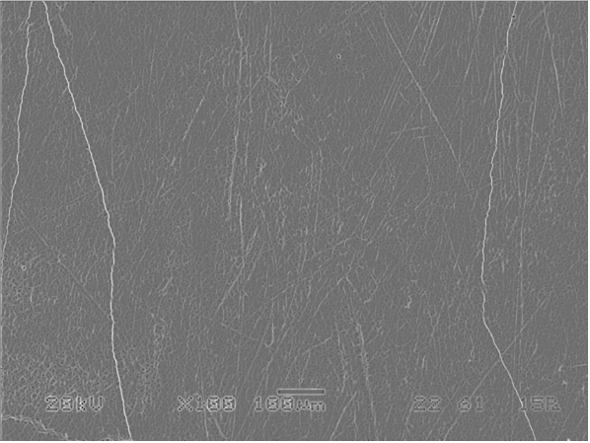
\includegraphics[width=.9\textwidth]{HessianaAutoLargos}
	\caption{Bordes usando HessianaAutoLargos}
	\end{subfigure}%
	
	\begin{subfigure}[c]{.5\linewidth}
	\centering\large 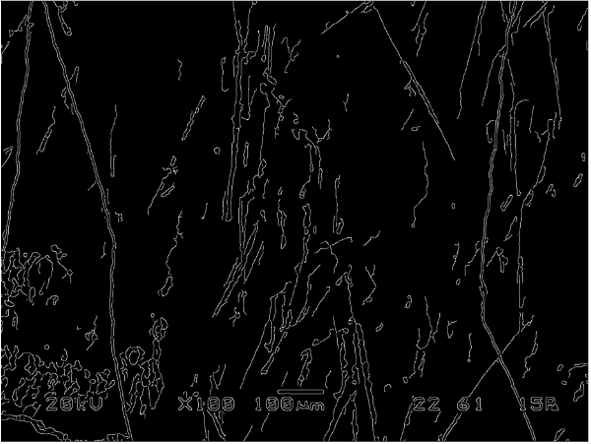
\includegraphics[width=.9\textwidth]{CannyP}
	\caption{Bordes usando CannyP}
	\end{subfigure}%
	\begin{subfigure}[c]{.5\linewidth}
	\centering\large 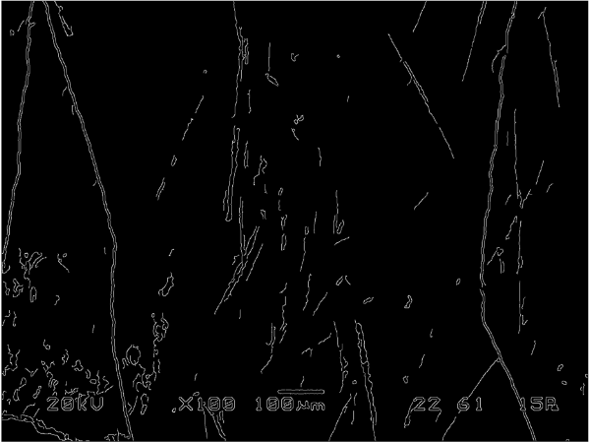
\includegraphics[width=.9\textwidth]{Canny}
	\caption{Bordes usando Canny}
	\end{subfigure}%
	
	\begin{subfigure}[c]{.5\linewidth}
	\centering\large 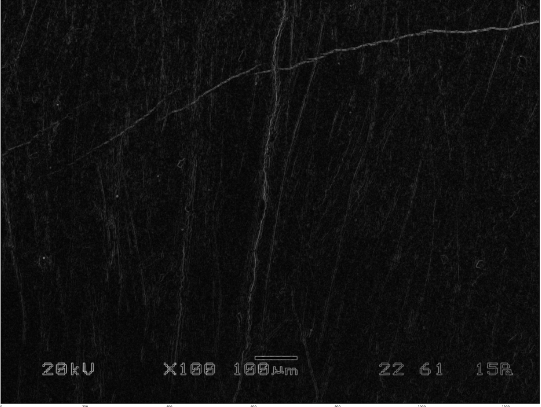
\includegraphics[width=.9\textwidth]{Kirsch}
	\caption{Bordes usando Kirsch}
	\end{subfigure}	

\caption{Resumen visual filtros usados.}\label{fig:1.1}
\end{figure}


\begin{figure}
	\begin{subfigure}[c]{.5\linewidth}
	\centering\large 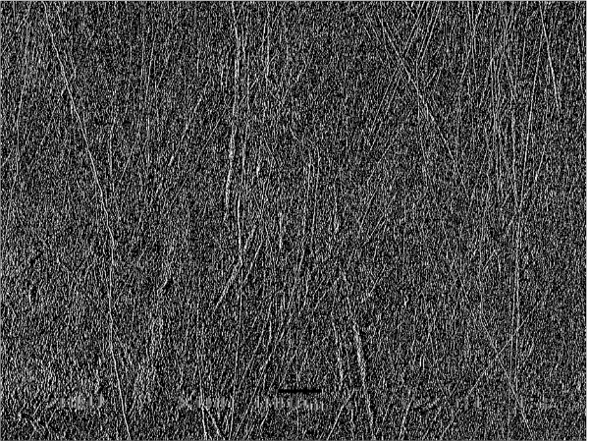
\includegraphics[width=.9\textwidth]{GaborI}
	\caption{Bordes usando Gabor filtro imaginario}
	\end{subfigure}%	
	\begin{subfigure}[c]{.5\linewidth}
	\centering\large 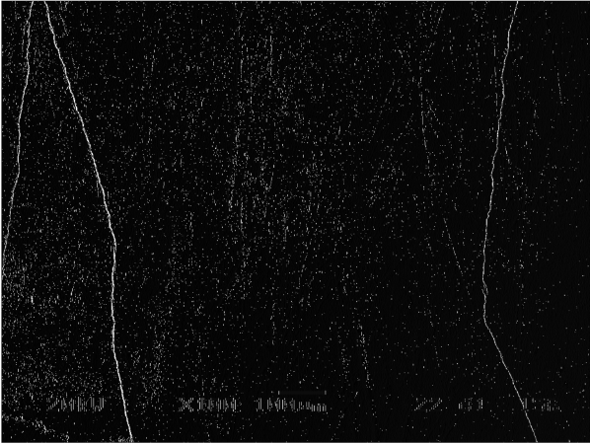
\includegraphics[width=.9\textwidth]{GaborR}
	\caption{Bordes usando Gabor filtro real}
	\end{subfigure}

\caption{Resumen visual filtros usados.}\label{fig:1.2}
\end{figure}



\begin{figure}

	\begin{subfigure}[c]{.5\linewidth}
	\centering\large 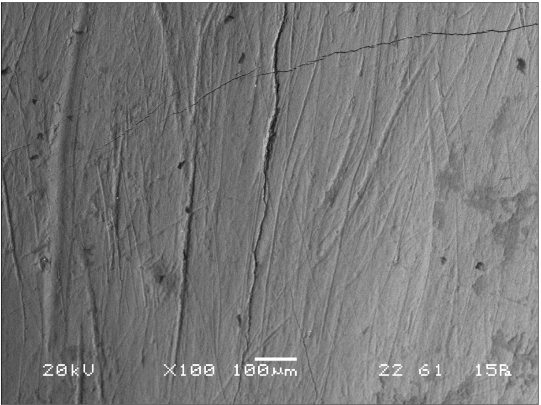
\includegraphics[width=.9\textwidth]{Imagen}
	\caption{Imagen original}
	\end{subfigure}%
	\begin{subfigure}[c]{.5\linewidth}
	\centering\large 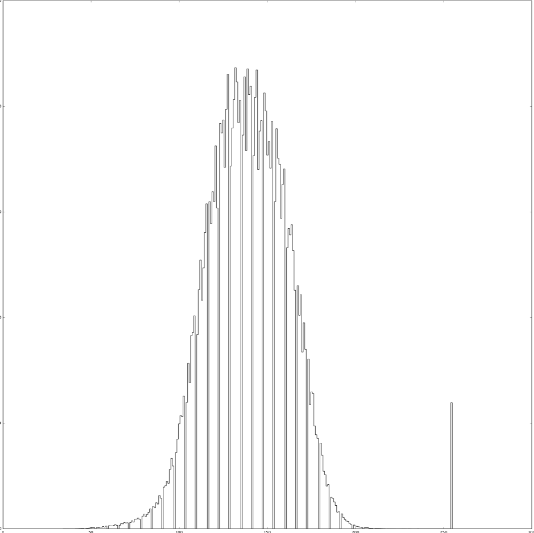
\includegraphics[width=.9\textwidth]{ImagenHist}
	\caption{Histograma imagen original}
	\end{subfigure}%	

	\begin{subfigure}[c]{.5\linewidth}
	\centering\large 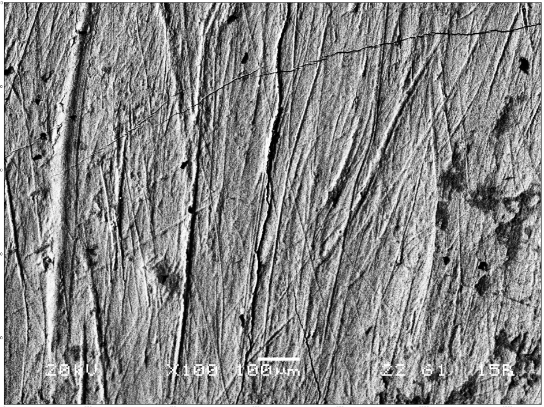
\includegraphics[width=.9\textwidth]{Equalized}
	\caption{Imagen ecualizada}
	\end{subfigure}%
	\begin{subfigure}[c]{.5\linewidth}
	\centering\large 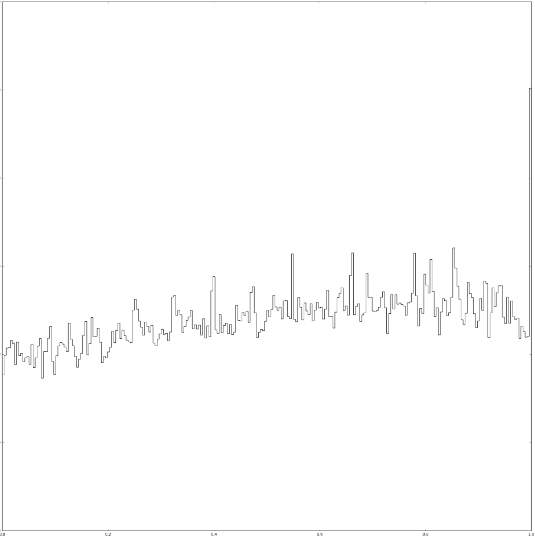
\includegraphics[width=.9\textwidth]{Histograma_Equali}
	\caption{Histograma imagen ecualizada}
	\end{subfigure}%

\caption{Pasos del procesado.}\label{fig:2.1}
\end{figure}

\begin{figure}
	\begin{subfigure}[c]{.5\linewidth}
	\centering\large 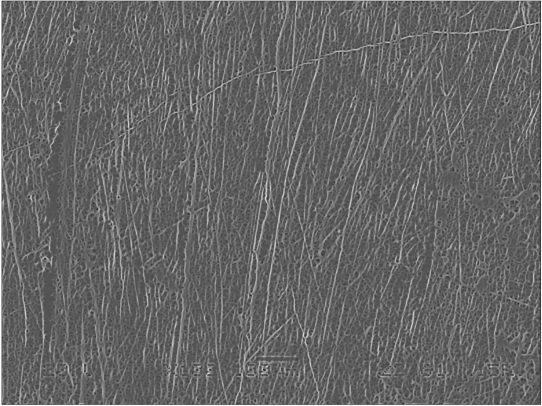
\includegraphics[width=.9\textwidth]{HessianaPaso2}
	\caption{Autovectores largos.}
	\end{subfigure}%
	\begin{subfigure}[c]{.5\linewidth}
	\centering\large 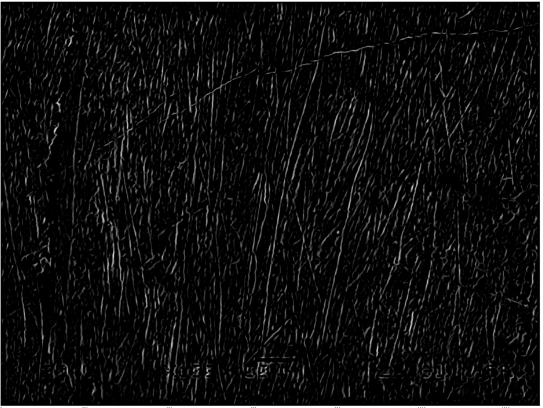
\includegraphics[width=.9\textwidth]{HessianaPaso2MenosFOndo}
	\caption{Hessiana menos fondo.}
	\end{subfigure}%	

	\begin{subfigure}[c]{.5\linewidth}
	\centering\large 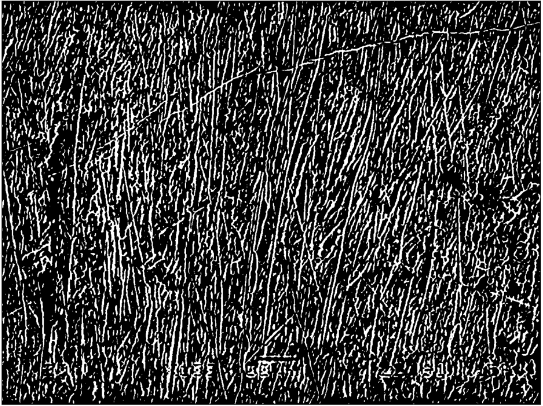
\includegraphics[width=.9\textwidth]{MenosFondoBinarizada}
	\caption{Binarizado.}
	\end{subfigure}%
	\begin{subfigure}[c]{.5\linewidth}
	\centering\large 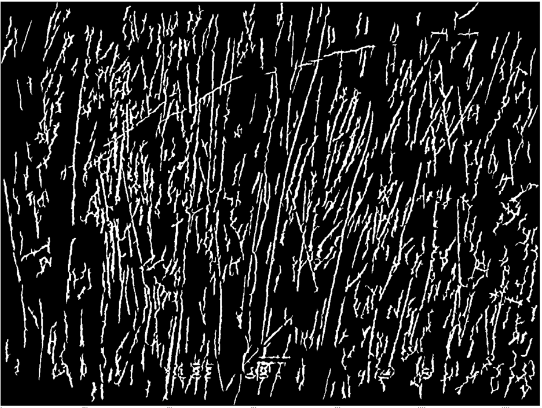
\includegraphics[width=.9\textwidth]{BinarizadaSinRuido}
	\caption{Binarizada sin ruido.}
	\end{subfigure}%

	\begin{subfigure}[c]{.5\linewidth}
	\centering\large 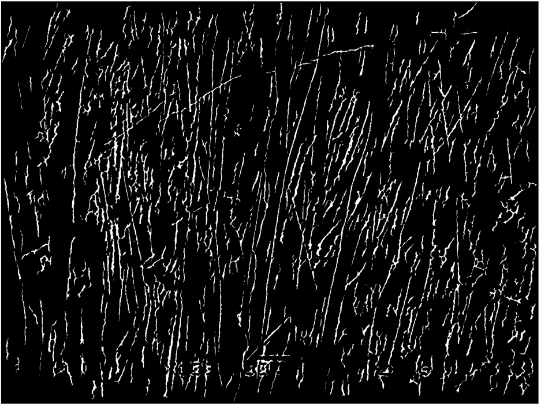
\includegraphics[width=.9\textwidth]{SinRuidoErosionada}
	\caption{Erosionado.}
	\end{subfigure}%
	\begin{subfigure}[c]{.5\linewidth}
	\centering\large 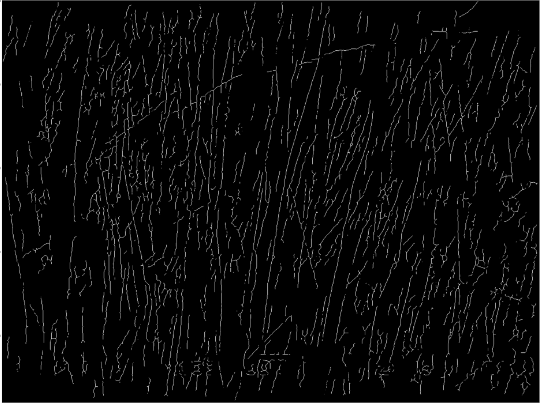
\includegraphics[width=.9\textwidth]{ErosionadaEsqueletonizada}
	\caption{Esqueletonizado de la erosión.}
	\end{subfigure}%
		
	\begin{subfigure}{.5\linewidth}
	\centering\large 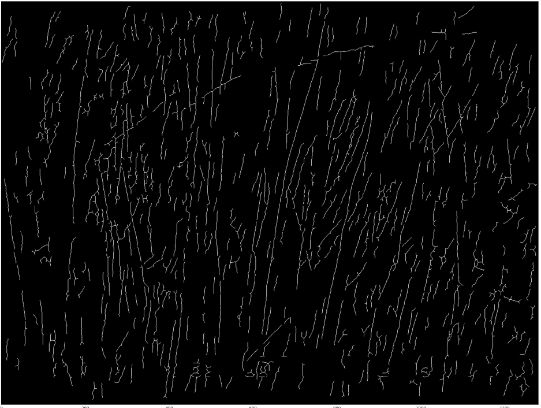
\includegraphics[width=.9\textwidth]{EsqueletonizadaSinRuido}
	\caption{Esqueletonizada sin ruido}
	\end{subfigure}%
	

\caption{Pasos del procesado.}\label{fig:2.2}
\end{figure}







\section{Por deep learning}
